% !TeX encoding = windows-1251
\documentclass[a4paper,12pt]{article}
\usepackage[mag=980]{newlistok}
\usepackage{tikz}

\УвеличитьВысоту{2.5cm}
\УвеличитьШирину{1.5cm}
%\renewcommand{\spacer}{\vfil}

\Заголовок{Самостоятельная работа}
\def\словоЛисток{СР \No\/}
\НомерЛистка{1$'$}
\ДатаЛистка{13 октября 2012г.}

\begin{document}


\ncopy{3}{
\vspace*{-12mm}
\СоздатьЗаголовок

\putthere{180mm}{-17mm}{%
    %
    %Картина для сумм треугольных чисел и т.п.
    %
      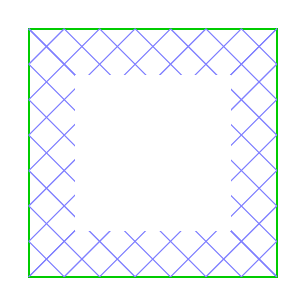
\begin{tikzpicture}
      [scale=.45
      ,fil/.style={color=green!50!white,opacity=.5}
      ,lin/.style={color=green!80!black,thick}
      ,lindot/.style={color=blue!50}
      ]
        \draw[lin] (0, 0) -- (7,0) -- (7,7) -- (0, 7) -- cycle;
        
        \foreach \i in {0,1,...,7}{
            \draw[lindot] (\i,0) -- (7, 7-\i);        
            \draw[lindot] (\i,0) -- (0, \i);        
            \draw[lindot] (\i,7) -- (7,  \i);        
            \draw[lindot] (\i,7) -- (0, 7-\i);        
        }
        \fill[color=white] (1.3, 1.3) -- (5.7,1.3) -- (5.7,5.7) -- (1.3, 5.7) -- cycle;
        
      \end{tikzpicture}
}{7cm}{}
\vspace{-4mm}


\УстановитьГраницы{0mm}{4truecm}
\задача
  Каждую сторону квадрата разбили на $n$ частей и через точки деления провели прямые, параллельные диагоналям квадрата. На сколько частей оказался разбит квадрат?
\кзадача


\задача
%  На Турнире городов было 5 задач. За каждую задачу можно получить одну из следующих оценок: $0$, $-$, $\mp$, %$\frac{+}{2}$, $\pm$, $+$. Всего на турнир пришло 1125 школьников. Обязательно ли среди их результатов есть одинаковые?
Дана арифметическая прогрессия из 11 членов. Сумма её членов с 5-ого по 7-ой равна 57. Найдите сумму всех членов прогрессии.
\кзадача

\ВосстановитьГраницы

\задача
Васе от дома до школы 10 остановок на автобусе.\\ (Вася живёт на остановке \лк0\пк, а школа находится на остановке \лк10\пк) Добирается до школы Вася следующим образом: он идёт пешком до тех пор, пока его не догонит автобус, тогда он в него садится. А в автобусе Вася едет, пока его не выгонит контроллёр. Второй раз садиться в автобус Вася уже не решается. Каким числом способов Вася может добраться до школы?
\кзадача


\задача
В шкафу 5 красных и 7 синих носков. Каким числом способов 3 человека могут одеть носки? (носки одного цвета считаются одинаковыми, однако левая нога отличается от правой)
\кзадача

\vspace*{-2mm}
\допраздел{* * *}
\vspace*{-3mm}

\сзадача
  Коля и Петя пришли в булочную. Там продаются булки 8 видов. Сколькими способами они могут купить себе по две булочки?
\кзадача
\hrl
\note{Для получения оценки $n$ необходимо правильно решить $n-1$ задачу. На переписывании оценку 5 можно получить только решив все 5 задач.
Можно пользоваться любыми своими записями и листочками. Доказывать всё.}
\vspace*{-4mm}
}


%\ЛичныйКондуит{0mm}{6mm}
%\СделатьКондуит{6mm}{6mm}

\end{document}
